\newcommand{\ausblickchapter}{Kapitel 9. }
\chapter{Ausblick}
\label{chapter:ausblick}
\lhead{\ausblickchapter \emph{Ausblick}}


%\section{Mögliche Erweiterungen}

%Es gibt einige Erweiterungsmöglichkeiten unserer Anwendung, welche wir im Rahmen dieses Projektes aus zeitlichen Gründen nicht umsetzen könnten, welche wir dennoch untersucht haben und deswegen nicht unerwähnt lassen möchten.
Wir haben im Rahmen unseres Bachelorprojektes gemerkt, dass Pepper in Kombination mit verschiedenen Frameworks und Tools zur Sammlung und Speicherung von Daten, ein enormes Erweiterungspotenzial bietet. Um auch auf die Möglichkeiten zum Ausbau unserer Arbeit aufzuzeigen, werden wir nun im Folgenden die für uns interessantesten Punkte darlegen.\\
\section{Google Dialogflow}

Dialog Flow ist eine von dem Konzern Google betriebene Plattform, welche das Verarbeiten und Verstehen von menschlicher Sprache ermöglicht. Sie bietet den Vorteil, dass die Verarbeitung der Sprache nicht mehr auf dem eigenen System stattfindet, sondern an einen von Google bereitgestellten Server gesendet wird. Dieser verarbeitet die Daten und sendet sie anschließend wieder zurück. Dialog Flow hat dabei den Vorteil, dass sich die Interaktion der Dialoge dynamisch auf der von Google erstellten Browser-Plattform bearbeiten lassen. Eine Implementierung in das Pepper System könnte so das produktive Arbeiten stark verbessern. Es ist außerdem möglich, Lernraten zu definieren, durch welche Pepper ohne das erneute Aufspielen einer Applikation dazu lernen könnte. Pepper wäre mit einer solchen Architektur in der Lage, selbst und dynamisch dazuzulernen und seine Interaktion und das Verstehen von Wörtern und Sprache ständig weiter zu optimieren. Wir haben für diese Funktionalität ein grafisches Konzept erstellt, welches den Ablauf dieser theoretischen Funktionalität verdeutlichen soll:

\begin{figure}[H]
    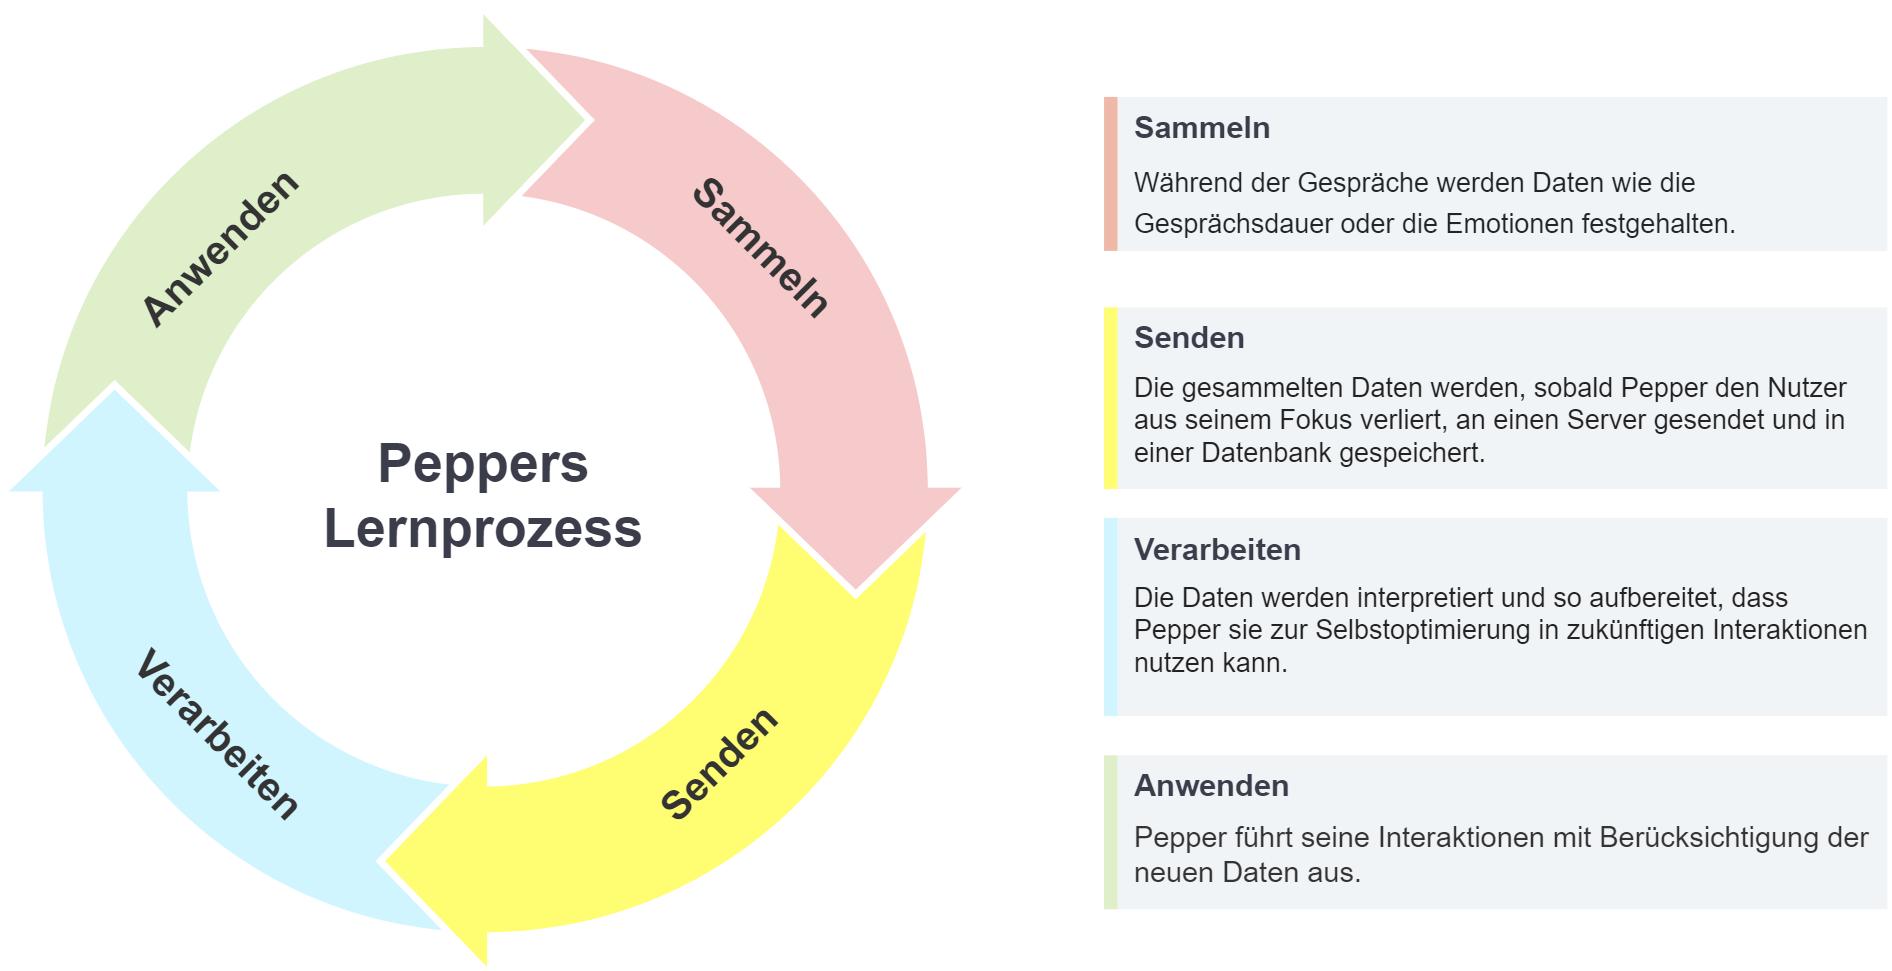
\includegraphics[width=\textwidth]{Figures/pepper-lerprozess.png}
    \caption{Diagramm: Lernprozess}
    \label{fig:integration}
    \centering
\end{figure}

Obwohl es eine von SoftBanks-Robotik offiziell bereitgestellte Schnittstelle für eine Anbindung an die Google-Dialogflow Plattform gibt, haben wir uns nicht nur aus zeitlichen Gründen gegen die Entwicklung einer solchen Funktionalität entschieden. Dabei gab es für uns zwei entscheidende Faktoren. Erstens empfinden wir es als äußerst unpassend, unser bereits entwickeltes System, welches dem Administrator den Vorteil bietet, die gesammelten Daten selbst zu besitzen, mit einer Anwendung zu verknüpfen, durch welche diese an einen Großkonzern weitergegeben werden. Das würde für uns bedeuten, dass wir einen unserer bedeutendsten Schwerpunkte dieser Arbeit verlieren, und zwar das ermöglichen gesammelte Daten selber zu verwalten und beliebig in eigene Dateiformate zu konvertieren und weiterzuverarbeiten. Außerdem ist es so, dass Google die Dialogflow Plattform nur für zahlende Kunden in Form eines Abo-Modells anbietet, wobei hier Mikrobeträge pro Request an die Plattform bezahlt werden müssen. Es wäre also alleine schon ein Kostenfaktor, eine Anwendung, während des Entwicklungsprozesses mit diesem System zu testen. Trotzdem möchten wir der Vollständigkeitshalber auf die Möglichkeit der Anbindung an Google Dialog hinweisen, auch wenn sie sich nicht mit den Ethischen-Vorstellungen unserer Softwareanwendung vereinbaren lassen.\\

\section{Dynamisches Bewegen im Raum}

Es ist möglich, Pepper das Bewegen in einem Raum beizubringen. Dies würde den Roboter für den Benutzer noch menschlicher erscheinen lassen, da es den Roboter um die Eigenschaft der Proxemik erweitern würde. Außerdem könnte Pepper so Routen ablaufen, um evtl. noch mehr Benutzer für die Interaktion zu finden und diese auf sich aufmerksam zu machen. Auch das automatische Ansteuern einer Ladestation wäre durch diese Funktion möglich, wodurch Pepper autonomer und noch unabhängiger von der Betreuung eines Menschen während seiner Arbeit wird.\\

\section{Socialmedia - Bot}
\label{sec:Sozialmedia-Bot}
Während der Arbeit an und mit Pepper fiel uns vor allem das außerordentliche Interesse auf, welches bei Passanten zu beobachten war. Es kam zudem des Öfteren vor, dass der Roboter gefilmt wurde oder man uns fragte, ob es möglich sei ein “Selfi” mit dem Roboter zu machen. Die von Pepper ausgelöste Neugier bei Menschen inspirierte uns zu dem Konzept, den Roboter selbst als Social-Media-Marketing Instrument einzusetzen. Ein solcher Anwendungsfall wäre durch die Implementierung eines oder mehrerer Bots (automatisierter Accounts) in die Architektur unserer Anwendung umsetzbar. Es wäre somit möglich, dass der Roboter bewusst Benutzer dazu auffordert, mit ihnen zu interagieren und ein Selbstporträt zu machen. Im Anschluss daran könnte der Bot mit einem zufällig gewählten Kommentar auf das veröffentlichte Bild regieren, wenn er erkennt, dass er auf diesem verlinkt wurde. Außerdem könnte der Bot selbstständig Veröffentlichungen aus den von ihm gesammelten Daten erstellen, in welchem er diese visuell darstellt und interpretiert. Pepper könnte so für seinen Besitzer einen positives Marketingeffekt erzielen.\\

\section{Weitere potenzielle Einsatzbereiche}

Wir haben während der Entwicklung mit Pepper noch eine Reihe weitere Anwendungsfälle für unsere Software-Architektur definiert. Drei dieser Einsatzbereiche haben wir im Folgendem aufgelistet.\\

\subsection{Gastronomie}

Es könnte ein System wie das aus dem Bachelor-Projekt mit Pepper als Möglichkeit zum Daten sammeln für die Gastronomie interessant sein. Pepper könnte Kunden zu ihrer Zufriedenheit befragen, Bestellungen aufnehmen oder über das Hygienekonzept informieren. Die dabei gesammelten Daten lassen sich flexibel analysieren, um ein genaueres Bild über die Kunden zu ermitteln und dies für potenzielle Optimierung von Geschäftsprozessen zu einzusetzen.\\

\subsection{Krankenhäuser und Pflegeeinrichtungen}

Pepper könnte viele zwischenmenschliche Aufgaben in einem Pflegeheim erfüllen. Zudem wäre es mit der von uns entwickelten Software-Architektur möglich, den gesundheitlichen Zustand und das generelle Wohlbefinden eines Bewohners einzuordnen und anschließend zu auf einem Server zu dokumentieren. Der Roboter könnte die Menschen in einer Einrichtung dabei spielerisch im Alltag unterstützen, während er Daten über die physische, sowie psychische Befindlichkeit sammelt. Wie die Daten können anschließend von Mitarbeitern des Pflegeheims ausgewertet werden.\\

\subsection{Kaufhäuser}

Große Einkaufszentren könnten die Anwendung ähnlich nutzen, wie wir es in unserem Entwurf für die Hochschule getan haben. Der Roboter würde Wegrouten beschreiben oder über das Kaufhaus informieren. Zusätzlich wäre es hier auch von Nutzen, den Roboter um ein Konzept wie in \ref{sec:Sozialmedia-Bot} beschrieben zu erweitern. Außerdem könnte Pepper so programmiert werden, dass er Anfragen zu spezifischen Produkten entgegennimmt, um dem Benutzer die entsprechenden Geschäfte zu nennen, in welchen es dieses zu erwerben gibt.\\

